%!TEX root = thesis.tex

\chapter{Methoden} % (fold)
\label{cha:methoden}

\section{Graphen} % (fold)
\label{sec:graphen}
Da die Breitensuche ein asymptotisch relativ schneller Algorithmus ist, sind relativ große Testgraphen nötig, um einigermaßen aussagekräftige Ergebnisse zu produzieren. Für diese Arbeit wurden Graphen in der Größenordnung von 100 000 Knoten gewählt. Diese wiederum relativ kleine Ausdehnung wurde gewählt, da der Testmodus beinhaltet, dass bei gleichbleibender Knotenanzahl die Dichte des Graphen variiert. Sehr dicht besiedelte Graphen mit 100 000 Knoten passen gerade noch in den Arbeitsspeicher. Würden noch größere Graphen verwendet, müsste entweder die Dichte des Graphen beschränkt werden oder das Betriebssysteme müsste Daten auslagern, was die Messergebnisse unbrauchbar machen würde. Da die asymptotische Laufzeit der Breitensuche aber O(n + m) ist \cite{SWB-283374373}, ist zu erwarten, dass bei gleicher (absoluter) Kantenzahl und erhöhter Knotenzahl, die Laufzeit nur leicht erhöht ist. Ein Beispiel: BFS auf einem Graph mit 1 000 000 Knoten und durchschnittlichem Knotengrad von 100 (ergibt 100 Mio Kanten) dauert nur leicht länger als die BFS auf einem Graph mit 100 000 Knoten und durchschnittlichem Knotengrad von 1000 (ergibt ebenso 100 Mio Kanten). Das liegt daran, dass zwar die reine Rechenzeit identisch ist, die zu versendenden Datenmengen aber größer werden, wenn der Graph mehr Knoten hat.

Es wurde ein Tool namens graph-generator \cite{graph-generator:2009:Online} eingesetzt, um zufällige Graphen zu generieren. Wie gesagt wurde als Knotenanzahl konstant 100 000 gewählt. Um einen Graph zu erstellen werden folgende Parameter gewählt:
\begin{description}
	\item[Minimaler Knotengrad min = 1] Der minimale Ausgangsgrad jedes Knotens.
	\item[Maximaler Knotengrad $max = \infty$] Der maximale Ausgangsgrad jedes Knotens.
	\item[Exponent exp = 5] Der Exponent der Exponentialverteiltung
	\item[Mittlerer Knotengrad z variiert]
\end{description}
Der Ausgangsgrad der Knoten ist folgendermaßen verteilt:
$$
P(X=k) \propto (k + offset)^{-exp}
$$
Der Offset wird dabei automatisch von dem Tool so gewählt, dass sich ein durchschnittlicher Ausgangsgrad von z ergibt.
% section graphen (end)

\section{Testplattformen} % (fold)
\label{sec:testplattform}
\begin{description}
	\item[Testplattform 1] Als Testplattform kann ein Apple Notebook von 2011 zum Einsatz. Es hat einen Intel Core i7-2720QM \enquote{Sandy Bridge} Prozessor, der mit 2.2Ghz getaktet wird. Es stehen 4 physikalische Kerne zur Verfügung, die jeweils Intels Hyper Threading Technologie unterstützen. Dadurch sind physikalisch 8 parallel laufende Threads möglich. Für den Vergleich sequentieller Algorithmen mit parallelen ist zu beachten, dass der Prozessor einen Kern auf bis zu 3.3 GHz übertakten kann, falls die anderen Kerne momentan nicht verwendet werden. Der optimal erreichbare Speedup ist demnach nicht 8.0, sondern deutlich darunter. Das Testsystem ist außerdem mit 8GB Hauptspeicher ausgestattet, der mit 1333MHz, der bei einem Takt von 1333Mhz arbeitet. Auf dem Testsystem wird als Betriebssystem Mac OS X 10.6.8 \enquote{Snow Leopard} und der x10 Compiler in der Version 2.2.3 verwendet.
	\item[Testplattform 2] Als zweiter Testrechner kam ein Desktop mit einem Intel Core i3-550 zum Einsatz. Die Takrate beträgt hier 3.2 GHz. Es stehen zwei Rechenkerne mit Hyper Threading, also 4 getrennte Ausführungsfäden zur Verfügung. Im System sind 2GB Hauptspeicher installiert. Als Betriebssystem wurde Ubuntu 12.04 verwendet. Der x10 Compiler wurde in der Version 2.2.3 verwendet. 

\end{description}
% section testplattform (end)

\section{Modus} % (fold)
\label{sec:modus}
Um Ergebnisse aus je einer Algorithmus - Graph - Kombination zu erhalten, wird der gewählte Algorithmus 3 mal auf dem gewählten Graph ausgeführt und die Zeit gemessen, die die reine Berechnung benötigte. Die Zeit, um den Graph in den Speicher einzulesen und die Daten auf die Places aufzuteilen, wurde nicht gemessen, da sie wenig mit dem Algorithmus und x10 zu tun hat. Die Zeit, die benötigt wird, um das Ergebnis von den beteiligten Places zurück zum Ursprungsplace zu holen, wird allerdings mitgemessen.

Wird ein x10 Programm mit der Umgebungsvariablen X10\_NPLACES gesetzt ausgeführt, werden die einzelnen Places durch Prozesse (nicht Threads) simuliert. Der Aufbau entspricht zwar nicht ganz dem Optimalsetup, in dem jeder Place einen physikalisch getrennten Speicherbereich repräsentiert, doch auch der Kontextwechsel, der bei der Kommunikation zwischen Places auftritt, ist relativ langsam und somit eine Annäherung an realen Kommunikationsoverhead. Trotzdem sind diese Ergebnisse nicht eins zu eins auf einen Rechnerverbund zu übertragen. Zum einen liegt das daran, dass, wie gesagt, die Kommunikation nochmal erheblich teurer wird, zum anderen können mit einem Rechnerverbund wesentlich größere Graphen bearbeitet werden, die offensichtlich ein viel höheres Potential zur Parallelisierung bieten. Andererseits dürfen die Ergebnisse dieser Arbeit auch nicht mit der lokalen Parallelisierung der Breitensuche auf einem einzelnen Rechner verwechselt werden. Kommunikation mittels geteiltem Speicher ist deutlich schneller, als die hier verwendete Inter-Prozess-Kommunikation. \\
Um die Möglichkeit der Parallelität zu messen, wurde der Algorithmus in der 1D und der 2D Zerlegung jeweils in einer Konfiguration mit 1, 2, 4, 8 und 9 Places ausgeführt. Die Konfiguration mit 9 Places wurden hinzugenommen, da so bei der 2D Zerlegung eine symmetrische 3 mal 3 Zerlegung stattfinden kann. Es wurde vermutet, dass eine quadratische Anzahl an Places besonders günstig für diesen Algorithmus sind. Der Vollständigkeit halber wurde auch der 1D Algorithmus mit 9 Places durchgeführt.

Um vollständige Ergebnisse zu bekommen, sollte eigentlich pro Graph die Breitensuche einmal von jedem Knoten aus gestartet werden. Allein diese Unterfangen würde den Zeitrahmen der kompletten Arbeit sprengen.     
% section modus (end)

\chapter{Ergebnisse und Diskussion} % (fold)
\label{cha:ergebnisse_und_diskussion}

Die vollständigen Messergebnisse finden sich in Anhang \ref{Anhang-Messwerte}. Wie bereits in Kapitel \ref{cha:methoden} beschrieben, wurde die Dichte des Graphen bei gleichbleibender Knotenanzahl erhöht. Sehr dünn besetzte Graphen waren deutlich schneller mit einer seriellen Version der Breitensuche zu lösen, als es mit jedwedem parallelen Algorithmus möglich war. Auch bei dichten Graphen war kein paralleler Algorithmus wirklich deutlich schneller. Der Vergleich der seriellen Breitensuche, mit der 1D-Breitensuche mit einem Place ist durchaus auch interessant. Um so mehr Kanten es gab, um so besser hat die 1D-Breitensuche abgeschnitten. Am langsamsten war in jedem Fall die 2D-Breitensuche.

\section{Serieller Fall, 1D mit einem Place und 2D mit einem Place} % (fold)
\label{sec:serieller_fall_vs_1d_mit_einem_place}
Jeder Algorithmus muss pro Iteration jeden aktiven Knoten mindestens einmal anfassen. Außerdem muss jeder Algorithmus pro Iteration jeden der Knoten mindestens einmal anfassen, der von einem der aktiven Knoten aus erreichbar ist. Der serielle Algorithmus tut genau das und nicht mehr. In Tests wurde herausgefunden, dass eine Iteration mittels einer herkömmlichen for-Schleife mit anschließendem direkten Zugriff mittels Index deutlich schneller ist (ca. 30\%), als eine foreach-Schleife. Der 1D-Algorithmus muss pro Iteration die Knoten in Sendepuffer einsortieren (jeden aktiven Knoten einmal anfassen), dann verschicken, was im Fall mit nur einem Place eine einfache Zeigerzuweisung ist. Anschließend muss dann nochmals jeder aktive Knoten angepasst werden, um alle erreichbaren Knoten zu erhalten. Der 1D-Algorithmus muss also zweimal über alle aktiven Knoten iterieren, zumindest in einer naiven Implementierung. Die verwendete optimierte Version legt diese beide Phasen aber zusammen. Zusätzliche Arbeit, im Gegensatz zu der seriellen Version, hat der 1D Algorithmus also nur beim Zurückkopieren des gesamten BFS-Distanz-Arrays. Die Messergebnisse zeigen, dass der serielle Algorithmus langsamer ist, als der 1D Algorithmus, wenn er mit nur einem Place gestartet wird. Nur bei sehr kleinen Graphe ist die Laufzeiten des seriellen Algorithmus ein Wenig schneller, da das Zurückkopieren des Arrays dann ausschlaggebend ist.

Wieso der serielle Algorithmus auf Listenbasis nicht, wie eigentlich erwartet, der schnellste ist, ist nicht ohne weiteres zu erklären. Zufall in Verbindung mit der Garbage Collection sind in Anbetracht der Deutlichkeit der Ergebnisse auszuschließen. Eine mögliche Erklärung ist, dass der Compiler den einen Code besser optimieren konnte, als den anderen, ohne dass sofort offensichtlich ist, woran das liegt.

Wie aus Abbildung \ref{Vergleich_Seriell} hervorgeht, ist der 2D Algorithmus deutlich langsamer als die beiden anderen. Der 2D Algorithmus hat 2 Kommunikationsphasen pro Iteration. In den beiden Phasen wir aber jeweils nur mit $\sqrt(p)$ anderen Places kommuniziert (bei p Places)\cite{Buluc:2011}, während im Fall des 1D Algorithmus jeder Place potentiell mit allen anderen kommuniziert. Im seriellen Fall ist diese zusätzliche Komplexität natürlich nicht nötig, verlangsamt aber den Ablauf.
% section serieller_fall_vs_1d_mit_einem_place (end)  

\begin{figure}
	\centering
	\label{Vergleich_Seriell}
	\caption{Vergleich der Laufzeiten bei serieller Ausführung, jeweils schnellste gemessene Laufzeit.}
	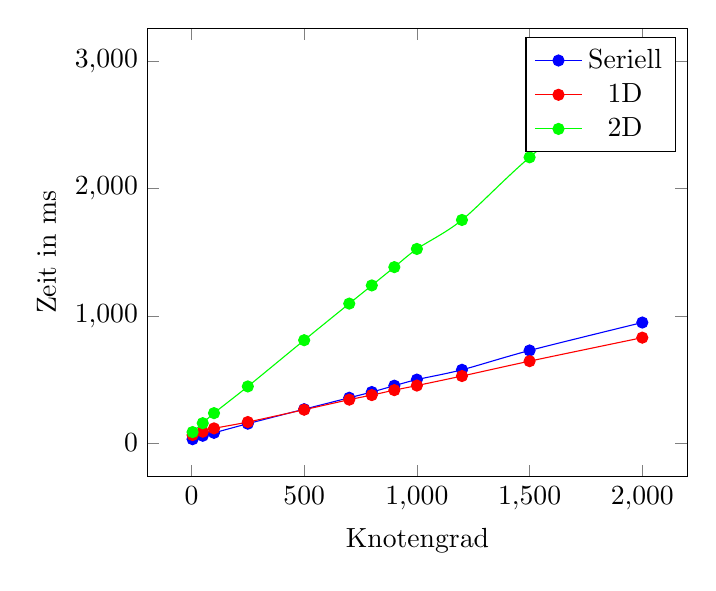
\begin{tikzpicture}
	    \begin{axis}[
	        xlabel=Knotengrad,
	        ylabel=Zeit in ms]
	    \addplot[smooth,mark=*,blue] plot coordinates {
	        (5,29)
	        (50,56)
	        (100,79)
	        (250,151)
	        (500,265)
	        (700,355)
	        (800,400)
	        (900,450)
	        (1000,498)
	        (1200,575)
	        (1500,727)
	        (2000,947)
	    };
	    \addlegendentry{Seriell}

	    \addplot[smooth,color=red,mark=*]
	        plot coordinates {
	        (5,62)
	        (50,88)
	        (100,114)
	        (250,164)
	        (500,261)
	        (700,340)
	        (800,376)
	        (900,415)
	        (1000,451)
	        (1200,526)
	        (1500,643)
	        (2000,828)
	        };
	    \addlegendentry{1D}

	    \addplot[smooth,color=green,mark=*]
	        plot coordinates {
	        (5,85)
	        (50,155)
	        (100,234)
	        (250,444)
	        (500,808)
	        (700,1096)
	        (800,1239)
	        (900,1383)
	        (1000,1526)
	        (1200,1754)
	        (1500,2247)
	        (2000, 2969)
	        };
	    \addlegendentry{2D}
	    \end{axis}
	\end{tikzpicture}
\end{figure}

\section{Ergebnisse der Parallelisierung} % (fold)
\label{sec:ergebnisse_der_parallelisierung}
Da die Breitensuche mit dem 2D Dekomposition keine vergleichbaren Ergebnisse lieferte, wird hier nur der serielle Algorithmus mit dem 1D Algorithmus verglichen. Mehr zu der 2D Breitensuche steht in Kapitel \ref{sec:die_2d_breitensuche}.
\begin{figure}
	\centering
	\begin{tikzpicture}
		\begin{axis}[nodes near coords,enlargelimits=0.2,width=450, height=250]
		    \addplot+[
		        point meta=explicit symbolic]
		    coordinates {
		        (5,1) [1]
		        (50,1) [1]
		        (100,1) [1]
		        (250,1) [1]
		        (500,0.29) [4]
		        (700,0.293) [4]
		        (800,0.294) [4]
		        (900,0.307) [4]
		        (1000,0.301) [4]
		        (1200,0.562) [4]
		        (1500,0.294) [4]
		        (2000,0.286) [4]
		    };
		    \addlegendentry{Effizienz}

		    \addplot+[
		        point meta=explicit symbolic]
		    coordinates {
		        (5,1) [1]
		        (50,1) [1]
		        (100,1) [1]
		        (250,1) [1]
		        (500,1.181) [4]
		        (700,1.172) [4]
		        (800,1.175) [4]
		        (900,1.228) [4]
			    (1000,1.203) [4]
			    (1200,2.248) [4]
			    (1500,1.178) [4]
			    (2000,1.142) [4]
			};
		    \addlegendentry{Speedup}
		    \addplot+[
		        point meta = none]
		    coordinates {
		    	(0,1)
		    	(2000,1)
		    };
		\end{axis}
	\end{tikzpicture}
\end{figure}
% section ergebnisse_der_parallelisierung (end)

\section{Die 2D Breitensuche} % (fold)
\label{sec:die_2d_breitensuche}
Die 2D Breitensuche ist in jedem Testfall der mit Abstand langsamste Algorithmus gewesen, was so nicht zu erwarten war. Der implementierte Algorithmus ist zwar zunächst deutlich komplexer, als die anderen beiden, doch gibt es zwei Vorteile, die diesen ALgorithmus gewiss studierenswert machen. Erstens sind die Gruppen von Places, die untereinander kommunizieren deutlich kleiner. In der ersten Kommunikationsphase sendet jeder Place seine Daten an eine ganze Spalte, und empfängt dafür von einer ganzen Zeile die Daten für den nächsten Schritt. Das sind $2 * \sqrt(p)$ Places, insgesamt, mit denen jeder Place kommunizieren muss, also $O(p * 2 + \sqrt(p) * \frac{1}{2}) = O(p * \sqrt(p))= O(p^{\frac{3}{2}})$ Kommunikationsvorgänge im System. In der zweiten Kommunikationsphase muss jeweils nur eine Zeile miteinander kommunizieren. Das sind zusätzlich $O(\sqrt(p) * p * \frac{1}{2})$ Kommunikationsvorgänge. Es sind also im O-Kalkül pro Iteration $O(p^{\frac{3}{2}})$. Im Vergleich dazu kommuniziert jeder Place im 1D Algorithmus mit allen anderen p-1 Places, also $O(p^2)$ Kommunikationsvorgänge. Der zweite Vorteil der Implementierung wie in \cite{Buluc:2011} ist die Möglichkeit, alle Kommunikation und Synchronisation auf drei MPI Operationen abzubilden. Die auf entsprechender Hardware vergleichsweise schnell sind. 

Beide dieser Vorteile sind bei der X10 Implementierung, die auf nur einem CPU läuft, hinfällig. Zunächst wurden die MPI Operationen in X10 \enquote{nachprogrammiert}. Um das zu tun, muss \textit{at} verwendet werden, dass einen für diesen Zweck unnützen Rückkanal hat. Bei der Verwendung einer hochperformanten MPI Hardware muss ein Datum nur einmal gesendet werden, wenn es an mehrere Empfänger gehen soll. Das ist in X10-Syntax nicht möglich. Die zusätzliche Kommunikation ist also teurer, als sie sein müsste. 
Der zweite Vorteil, eben dass weniger Kommunikationsvorgänge im System sind, ist aus zwei Gründen hier nicht ausschlaggebend. Zum einen sind dermaßen wenig Places im Spiel, dass die Zahlen sich fast gleichen, zum anderen haben erste Tests gezeigt, dass die Kommunikationsphasen etwa 4 bis 5 Mal so schnell sind wie die Rechenphasen, also die Kommunikation nicht so ausschlaggebend ist, wie das zu erwarten war. Das wiederum ist auf die Testumgebung ohne wirklich getrennte Places zurückzuführen.

Wie in \cite{Buluc:2011} ist also die 2D Implementierung eher die schlechtere, wobei in den Dimensionen, in denen in dieser Arbeit gedacht wird,  die Unterschiede gravierender sind. Ob in  größeren Testumgebungen die Ergebnisse anders ausfallen, muss in einer weiteren Arbeit untersucht werden.
% section die_2d_breitensuche (end)
% chapter ergebnisse_und_diskussion (end)